\documentclass[]{article}

\usepackage{listings}
\usepackage{mathtools}
\usepackage{multirow}

\title{Introduction to Intelligent Systems \\ Project1: Rolling Die Mazes}
\author{Joseph Fuchs, Damien Cremilleux}

\begin{document}
\maketitle

\section{Problem definition}
The objective of this project is to solve rolling-die mazes.
A  die start from a location on the maze, and can roll along its edges through a grid, until a goal location is found.
The mazes can contain obstacles, and there are restrictions on which numbers may face up on the die.
The die will always start with the 1 facing up ('visible'), 2 facing up/north, and 3 to the right/east.
Moreover, the number 6 should never be face up on the die, and the number 1 must be on top of the die when the goal location is reached.

\medskip

An example of maze is given below (S is the start location, G is the goal location and * are obstacles).

\lstinputlisting[]{../puzzles/puzzle4.txt}

\medskip

This problem can be formulated as follow:
\begin{itemize}
\item States: The state is determined by both the die position and its orientation.
So, a states description specifies the location (ie the coordinates) and the orientation (which number is facing up, north and east) of the dice on the maze.
\item Initial state: The die is on the start location, with the 1 facing up.
\item Actions: Rolling north, south, east or west. Different subsets of these are possible depending on the orientation of the dice (the number 6 should never be face up).
\item Transitions model: Given a state and action, this return the resulting state.
\item Goal test: The die is on the goal location, with the number 1 on the top.
\item Path cost: Each step costs 1, so the path cost is the number of steps in the path.
\end{itemize}

\section{Heuristics}
We use A* algorithm (discussed in the class) to solve this search problem.
A* includes as a component of its evaluation function a heuristic function, $h(n)$.
In the following sections, we describe the three heuristics chosen to solve this search problem.

\subsection{Uniform-cost search}
For the first heuristic, $h_1$, we chose a very simple solution: $h(n) = 0$.
This means that the evaluation function is now $f(n) = g(n)$ where $g(n)$ is the cost to reach the node.
With this heuristic, we have an uniform-cost search algorithm.
Uniform-cost search first visits the node with the shortest path costs from the root node.

This heuristic is admissible.
It will never overestimate the cost to reach the goal because the heuristic is equal to 0, and we are dealing with positive step costs.

Moreover this heuristic is consistent, which is a stricter requirement than admissibility.
According to the textbook, a heuristic is consistent if, for every node $n$ and every successor $n’$ of n generated by any action $a$, the estimated cost of reaching the goal from $n$ is no greater than the step cost of getting to $n’$ plus the estimated cost of reaching the goal from $n’$:

$
h(n) \leq c(n,a,n’) + h(n,)

0 \leq c(n,a,n’)
$

This is true because we are dealing with positive step costs.

\subsection{Manhattan distance without obstacles}
The second heuristic, $h_2$, is based on the city block distance, or Manhattan distance, which is the sum of the absolute differences of Cartesian coordinates.
To find this heuristic, we take the original problem with fewer restrictions: no obstacles and we do not take into account what is the orientation of the die. 
We illustrate this on the following maze.
The die is on the cell marked ‘D’.
In this case, the heuristic will be $h(n=’D’) = 4$.

\begin{lstlisting}
S . . . .
D . * * *
. * . . G
. . . . .
* . . . .
\end{lstlisting}

So this is a relaxed problem of the first one.
We know that the cost of an optimal solution to a relaxed problem is an admissible heuristic for the original problem.
Moreover, this heuristic is also consistent, because it is the exact cost for the relaxed problem so it must obey the triangle inequality.
Finally, this heuristic gives bigger values than h1. This means that we can expect better results with this heuristics, compare to the previous one. 


\subsection{Manhattan distance with orientation}
For the last heuristic, $h_3$, we also generate an heuristic from a relaxed problem.
We know only ignore the restriction about the obstacles.
Contrary to the heuristic two, we take the orientation of the die into consideration.
Given the position and the orientation of the dice, it is possible to find a minimal number of rotations to do to solve the maze.
For instance, if the die with the 1 on top is on the same row or column as the goal position, the maze can be solve in $mahattan\_distance + 2$.

So we can generate a set of rules giving the position and orientation.
We observe that each time the rule has the form  $mahattan\_distance + cst$, the value given by $h_3$ will be at least as big as $h_2$ for all nodes.
This heuristic is likely to be more effective than the previous one.
We illustrate this heuristic with the following maze.
Now the heuristic will be $h_3(n=’D’) = 4 + 2 = 6$.

\begin{lstlisting}
S . . . .
. . * * *
D * . . G
. . . . .
* . . . .
\end{lstlisting}

We again used a relaxed problem of the original one.
For the same reasons like $h_2$, this heuristic is admissible and consistent.

\section{Performance metrics}

For each heuristics, we ran the five puzzles given in the wording.
The results are in the following tables.

\begin{center}
    \begin{tabular}{| c | c | c | c | c | c | c | c | c | c | c |}
      \cline{2-10} & \multicolumn{3}{|c|}{Puzzle 1} & \multicolumn{3}{|c|}{Puzzle 2} & \multicolumn{3}{|c|}{Puzzle 3} \\
      \hline
    & $h_1$ & $h_2$ & $h_3$ & $h_1$ & $h_2$& $h_3$ & $h_1$ &  $h_2$ & $h_3$ \\ \hline
    Number of nodes generated & 32 & 12 &  & 95 & 67 &  & 2 & 2 & \\ \hline
    Number of nodes visited   & 24 & 9  &  & 84 & 50 &  & 3 & 3 & \\ \hline
    \end{tabular}
\end{center}

\begin{center}
    \begin{tabular}{| c | c | c | c | c | c | c | c |}
      \cline{2-7} & \multicolumn{3}{|c|}{Puzzle 4} & \multicolumn{3}{|c|}{Puzzle 5} \\
      \hline
    & $h_1$ & $h_2$ & $h_3$ & $h_1$ & $h_2$& $h_3$ \\ \hline
    Number of nodes generated & 161 & 101 &       & 1271 & 1080 &   \\ \hline
    Number of nodes visited   & 149 & 82  &       & 1260 &  737 &  \\ \hline
    \end{tabular}
\end{center}

To show the difference, the following bar graphs give the number of nodes generated and visited according to the heuristic, for each puzzle.

% GNUPLOT: LaTeX picture with Postscript
\begingroup
  \makeatletter
  \providecommand\color[2][]{%
    \GenericError{(gnuplot) \space\space\space\@spaces}{%
      Package color not loaded in conjunction with
      terminal option `colourtext'%
    }{See the gnuplot documentation for explanation.%
    }{Either use 'blacktext' in gnuplot or load the package
      color.sty in LaTeX.}%
    \renewcommand\color[2][]{}%
  }%
  \providecommand\includegraphics[2][]{%
    \GenericError{(gnuplot) \space\space\space\@spaces}{%
      Package graphicx or graphics not loaded%
    }{See the gnuplot documentation for explanation.%
    }{The gnuplot epslatex terminal needs graphicx.sty or graphics.sty.}%
    \renewcommand\includegraphics[2][]{}%
  }%
  \providecommand\rotatebox[2]{#2}%
  \@ifundefined{ifGPcolor}{%
    \newif\ifGPcolor
    \GPcolorfalse
  }{}%
  \@ifundefined{ifGPblacktext}{%
    \newif\ifGPblacktext
    \GPblacktexttrue
  }{}%
  % define a \g@addto@macro without @ in the name:
  \let\gplgaddtomacro\g@addto@macro
  % define empty templates for all commands taking text:
  \gdef\gplbacktext{}%
  \gdef\gplfronttext{}%
  \makeatother
  \ifGPblacktext
    % no textcolor at all
    \def\colorrgb#1{}%
    \def\colorgray#1{}%
  \else
    % gray or color?
    \ifGPcolor
      \def\colorrgb#1{\color[rgb]{#1}}%
      \def\colorgray#1{\color[gray]{#1}}%
      \expandafter\def\csname LTw\endcsname{\color{white}}%
      \expandafter\def\csname LTb\endcsname{\color{black}}%
      \expandafter\def\csname LTa\endcsname{\color{black}}%
      \expandafter\def\csname LT0\endcsname{\color[rgb]{1,0,0}}%
      \expandafter\def\csname LT1\endcsname{\color[rgb]{0,1,0}}%
      \expandafter\def\csname LT2\endcsname{\color[rgb]{0,0,1}}%
      \expandafter\def\csname LT3\endcsname{\color[rgb]{1,0,1}}%
      \expandafter\def\csname LT4\endcsname{\color[rgb]{0,1,1}}%
      \expandafter\def\csname LT5\endcsname{\color[rgb]{1,1,0}}%
      \expandafter\def\csname LT6\endcsname{\color[rgb]{0,0,0}}%
      \expandafter\def\csname LT7\endcsname{\color[rgb]{1,0.3,0}}%
      \expandafter\def\csname LT8\endcsname{\color[rgb]{0.5,0.5,0.5}}%
    \else
      % gray
      \def\colorrgb#1{\color{black}}%
      \def\colorgray#1{\color[gray]{#1}}%
      \expandafter\def\csname LTw\endcsname{\color{white}}%
      \expandafter\def\csname LTb\endcsname{\color{black}}%
      \expandafter\def\csname LTa\endcsname{\color{black}}%
      \expandafter\def\csname LT0\endcsname{\color{black}}%
      \expandafter\def\csname LT1\endcsname{\color{black}}%
      \expandafter\def\csname LT2\endcsname{\color{black}}%
      \expandafter\def\csname LT3\endcsname{\color{black}}%
      \expandafter\def\csname LT4\endcsname{\color{black}}%
      \expandafter\def\csname LT5\endcsname{\color{black}}%
      \expandafter\def\csname LT6\endcsname{\color{black}}%
      \expandafter\def\csname LT7\endcsname{\color{black}}%
      \expandafter\def\csname LT8\endcsname{\color{black}}%
    \fi
  \fi
  \setlength{\unitlength}{0.0500bp}%
  \begin{picture}(7200.00,5040.00)%
    \gplgaddtomacro\gplbacktext{%
      \csname LTb\endcsname%
      \put(594,440){\makebox(0,0)[r]{\strut{} 5}}%
      \put(594,1097){\makebox(0,0)[r]{\strut{} 10}}%
      \put(594,1753){\makebox(0,0)[r]{\strut{} 15}}%
      \put(594,2410){\makebox(0,0)[r]{\strut{} 20}}%
      \put(594,3066){\makebox(0,0)[r]{\strut{} 25}}%
      \put(594,3723){\makebox(0,0)[r]{\strut{} 30}}%
      \put(594,4379){\makebox(0,0)[r]{\strut{} 35}}%
      \put(2752,220){\makebox(0,0){\strut{}Nodes visited}}%
      \put(4777,220){\makebox(0,0){\strut{}Nodes generated}}%
      \put(3764,4709){\makebox(0,0){\strut{}Results for puzzle 1}}%
    }%
    \gplgaddtomacro\gplfronttext{%
      \csname LTb\endcsname%
      \put(5816,4206){\makebox(0,0)[r]{\strut{}h1}}%
      \csname LTb\endcsname%
      \put(5816,3986){\makebox(0,0)[r]{\strut{}h2}}%
      \csname LTb\endcsname%
      \put(5816,3766){\makebox(0,0)[r]{\strut{}h3}}%
    }%
    \gplbacktext
    \put(0,0){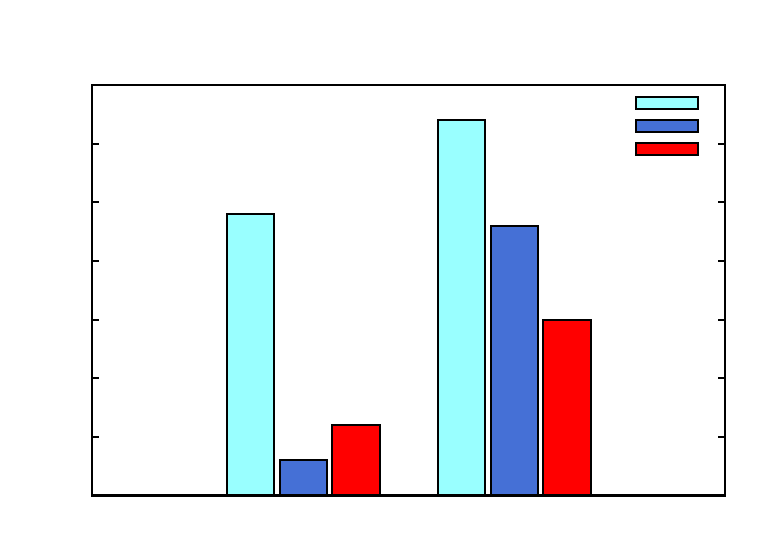
\includegraphics{graph1}}%
    \gplfronttext
  \end{picture}%
\endgroup


% GNUPLOT: LaTeX picture with Postscript
\begingroup
  \makeatletter
  \providecommand\color[2][]{%
    \GenericError{(gnuplot) \space\space\space\@spaces}{%
      Package color not loaded in conjunction with
      terminal option `colourtext'%
    }{See the gnuplot documentation for explanation.%
    }{Either use 'blacktext' in gnuplot or load the package
      color.sty in LaTeX.}%
    \renewcommand\color[2][]{}%
  }%
  \providecommand\includegraphics[2][]{%
    \GenericError{(gnuplot) \space\space\space\@spaces}{%
      Package graphicx or graphics not loaded%
    }{See the gnuplot documentation for explanation.%
    }{The gnuplot epslatex terminal needs graphicx.sty or graphics.sty.}%
    \renewcommand\includegraphics[2][]{}%
  }%
  \providecommand\rotatebox[2]{#2}%
  \@ifundefined{ifGPcolor}{%
    \newif\ifGPcolor
    \GPcolorfalse
  }{}%
  \@ifundefined{ifGPblacktext}{%
    \newif\ifGPblacktext
    \GPblacktexttrue
  }{}%
  % define a \g@addto@macro without @ in the name:
  \let\gplgaddtomacro\g@addto@macro
  % define empty templates for all commands taking text:
  \gdef\gplbacktext{}%
  \gdef\gplfronttext{}%
  \makeatother
  \ifGPblacktext
    % no textcolor at all
    \def\colorrgb#1{}%
    \def\colorgray#1{}%
  \else
    % gray or color?
    \ifGPcolor
      \def\colorrgb#1{\color[rgb]{#1}}%
      \def\colorgray#1{\color[gray]{#1}}%
      \expandafter\def\csname LTw\endcsname{\color{white}}%
      \expandafter\def\csname LTb\endcsname{\color{black}}%
      \expandafter\def\csname LTa\endcsname{\color{black}}%
      \expandafter\def\csname LT0\endcsname{\color[rgb]{1,0,0}}%
      \expandafter\def\csname LT1\endcsname{\color[rgb]{0,1,0}}%
      \expandafter\def\csname LT2\endcsname{\color[rgb]{0,0,1}}%
      \expandafter\def\csname LT3\endcsname{\color[rgb]{1,0,1}}%
      \expandafter\def\csname LT4\endcsname{\color[rgb]{0,1,1}}%
      \expandafter\def\csname LT5\endcsname{\color[rgb]{1,1,0}}%
      \expandafter\def\csname LT6\endcsname{\color[rgb]{0,0,0}}%
      \expandafter\def\csname LT7\endcsname{\color[rgb]{1,0.3,0}}%
      \expandafter\def\csname LT8\endcsname{\color[rgb]{0.5,0.5,0.5}}%
    \else
      % gray
      \def\colorrgb#1{\color{black}}%
      \def\colorgray#1{\color[gray]{#1}}%
      \expandafter\def\csname LTw\endcsname{\color{white}}%
      \expandafter\def\csname LTb\endcsname{\color{black}}%
      \expandafter\def\csname LTa\endcsname{\color{black}}%
      \expandafter\def\csname LT0\endcsname{\color{black}}%
      \expandafter\def\csname LT1\endcsname{\color{black}}%
      \expandafter\def\csname LT2\endcsname{\color{black}}%
      \expandafter\def\csname LT3\endcsname{\color{black}}%
      \expandafter\def\csname LT4\endcsname{\color{black}}%
      \expandafter\def\csname LT5\endcsname{\color{black}}%
      \expandafter\def\csname LT6\endcsname{\color{black}}%
      \expandafter\def\csname LT7\endcsname{\color{black}}%
      \expandafter\def\csname LT8\endcsname{\color{black}}%
    \fi
  \fi
  \setlength{\unitlength}{0.0500bp}%
  \begin{picture}(7200.00,5040.00)%
    \gplgaddtomacro\gplbacktext{%
      \csname LTb\endcsname%
      \put(594,440){\makebox(0,0)[r]{\strut{} 0}}%
      \put(594,855){\makebox(0,0)[r]{\strut{} 10}}%
      \put(594,1269){\makebox(0,0)[r]{\strut{} 20}}%
      \put(594,1684){\makebox(0,0)[r]{\strut{} 30}}%
      \put(594,2099){\makebox(0,0)[r]{\strut{} 40}}%
      \put(594,2513){\makebox(0,0)[r]{\strut{} 50}}%
      \put(594,2928){\makebox(0,0)[r]{\strut{} 60}}%
      \put(594,3342){\makebox(0,0)[r]{\strut{} 70}}%
      \put(594,3757){\makebox(0,0)[r]{\strut{} 80}}%
      \put(594,4172){\makebox(0,0)[r]{\strut{} 90}}%
      \put(2752,220){\makebox(0,0){\strut{}Nodes visited}}%
      \put(4777,220){\makebox(0,0){\strut{}Nodes generated}}%
      \put(3764,4709){\makebox(0,0){\strut{}Results for puzzle 2}}%
    }%
    \gplgaddtomacro\gplfronttext{%
      \csname LTb\endcsname%
      \put(5816,4206){\makebox(0,0)[r]{\strut{}h1}}%
      \csname LTb\endcsname%
      \put(5816,3986){\makebox(0,0)[r]{\strut{}h2}}%
      \csname LTb\endcsname%
      \put(5816,3766){\makebox(0,0)[r]{\strut{}h3}}%
    }%
    \gplbacktext
    \put(0,0){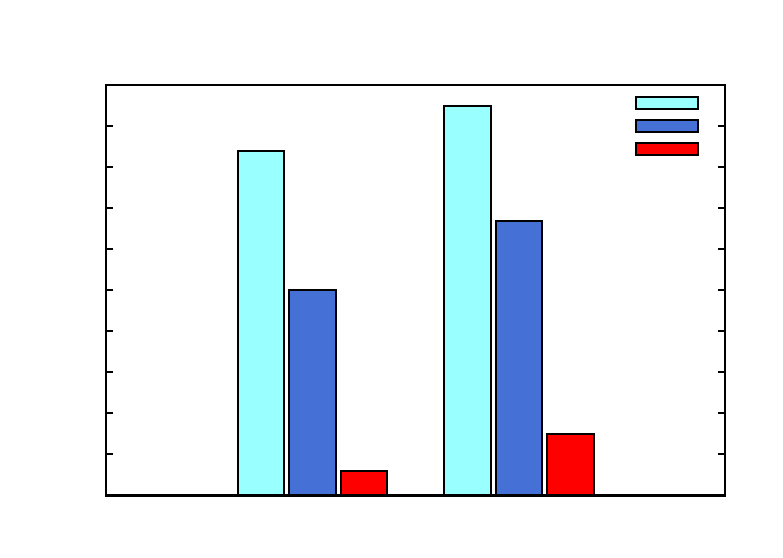
\includegraphics{graph2}}%
    \gplfronttext
  \end{picture}%
\endgroup


% GNUPLOT: LaTeX picture with Postscript
\begingroup
  \makeatletter
  \providecommand\color[2][]{%
    \GenericError{(gnuplot) \space\space\space\@spaces}{%
      Package color not loaded in conjunction with
      terminal option `colourtext'%
    }{See the gnuplot documentation for explanation.%
    }{Either use 'blacktext' in gnuplot or load the package
      color.sty in LaTeX.}%
    \renewcommand\color[2][]{}%
  }%
  \providecommand\includegraphics[2][]{%
    \GenericError{(gnuplot) \space\space\space\@spaces}{%
      Package graphicx or graphics not loaded%
    }{See the gnuplot documentation for explanation.%
    }{The gnuplot epslatex terminal needs graphicx.sty or graphics.sty.}%
    \renewcommand\includegraphics[2][]{}%
  }%
  \providecommand\rotatebox[2]{#2}%
  \@ifundefined{ifGPcolor}{%
    \newif\ifGPcolor
    \GPcolorfalse
  }{}%
  \@ifundefined{ifGPblacktext}{%
    \newif\ifGPblacktext
    \GPblacktexttrue
  }{}%
  % define a \g@addto@macro without @ in the name:
  \let\gplgaddtomacro\g@addto@macro
  % define empty templates for all commands taking text:
  \gdef\gplbacktext{}%
  \gdef\gplfronttext{}%
  \makeatother
  \ifGPblacktext
    % no textcolor at all
    \def\colorrgb#1{}%
    \def\colorgray#1{}%
  \else
    % gray or color?
    \ifGPcolor
      \def\colorrgb#1{\color[rgb]{#1}}%
      \def\colorgray#1{\color[gray]{#1}}%
      \expandafter\def\csname LTw\endcsname{\color{white}}%
      \expandafter\def\csname LTb\endcsname{\color{black}}%
      \expandafter\def\csname LTa\endcsname{\color{black}}%
      \expandafter\def\csname LT0\endcsname{\color[rgb]{1,0,0}}%
      \expandafter\def\csname LT1\endcsname{\color[rgb]{0,1,0}}%
      \expandafter\def\csname LT2\endcsname{\color[rgb]{0,0,1}}%
      \expandafter\def\csname LT3\endcsname{\color[rgb]{1,0,1}}%
      \expandafter\def\csname LT4\endcsname{\color[rgb]{0,1,1}}%
      \expandafter\def\csname LT5\endcsname{\color[rgb]{1,1,0}}%
      \expandafter\def\csname LT6\endcsname{\color[rgb]{0,0,0}}%
      \expandafter\def\csname LT7\endcsname{\color[rgb]{1,0.3,0}}%
      \expandafter\def\csname LT8\endcsname{\color[rgb]{0.5,0.5,0.5}}%
    \else
      % gray
      \def\colorrgb#1{\color{black}}%
      \def\colorgray#1{\color[gray]{#1}}%
      \expandafter\def\csname LTw\endcsname{\color{white}}%
      \expandafter\def\csname LTb\endcsname{\color{black}}%
      \expandafter\def\csname LTa\endcsname{\color{black}}%
      \expandafter\def\csname LT0\endcsname{\color{black}}%
      \expandafter\def\csname LT1\endcsname{\color{black}}%
      \expandafter\def\csname LT2\endcsname{\color{black}}%
      \expandafter\def\csname LT3\endcsname{\color{black}}%
      \expandafter\def\csname LT4\endcsname{\color{black}}%
      \expandafter\def\csname LT5\endcsname{\color{black}}%
      \expandafter\def\csname LT6\endcsname{\color{black}}%
      \expandafter\def\csname LT7\endcsname{\color{black}}%
      \expandafter\def\csname LT8\endcsname{\color{black}}%
    \fi
  \fi
  \setlength{\unitlength}{0.0500bp}%
  \begin{picture}(7200.00,5040.00)%
    \gplgaddtomacro\gplbacktext{%
      \csname LTb\endcsname%
      \put(594,440){\makebox(0,0)[r]{\strut{} 2}}%
      \put(594,1003){\makebox(0,0)[r]{\strut{} 4}}%
      \put(594,1565){\makebox(0,0)[r]{\strut{} 6}}%
      \put(594,2128){\makebox(0,0)[r]{\strut{} 8}}%
      \put(594,2691){\makebox(0,0)[r]{\strut{} 10}}%
      \put(594,3254){\makebox(0,0)[r]{\strut{} 12}}%
      \put(594,3816){\makebox(0,0)[r]{\strut{} 14}}%
      \put(594,4379){\makebox(0,0)[r]{\strut{} 16}}%
      \put(2752,220){\makebox(0,0){\strut{}Nodes visited}}%
      \put(4777,220){\makebox(0,0){\strut{}Nodes generated}}%
      \put(3764,4709){\makebox(0,0){\strut{}Results for puzzle 3}}%
    }%
    \gplgaddtomacro\gplfronttext{%
      \csname LTb\endcsname%
      \put(5816,4206){\makebox(0,0)[r]{\strut{}h1}}%
      \csname LTb\endcsname%
      \put(5816,3986){\makebox(0,0)[r]{\strut{}h2}}%
      \csname LTb\endcsname%
      \put(5816,3766){\makebox(0,0)[r]{\strut{}h3}}%
    }%
    \gplbacktext
    \put(0,0){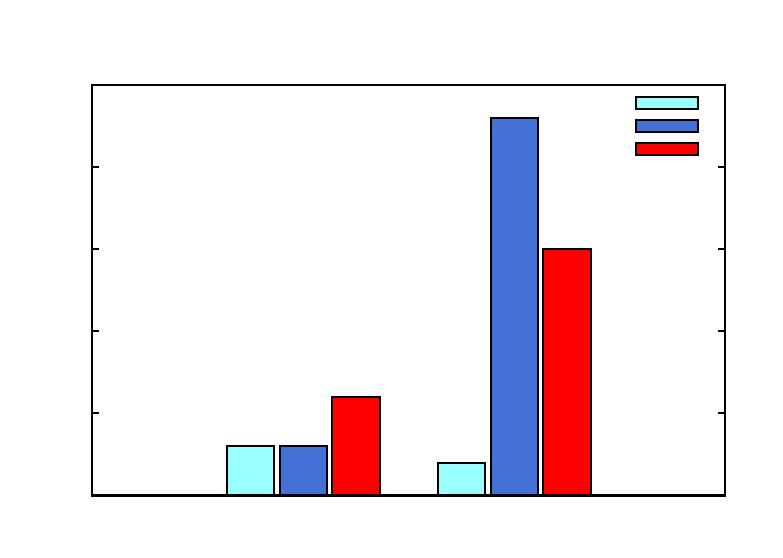
\includegraphics{graph3}}%
    \gplfronttext
  \end{picture}%
\endgroup


% GNUPLOT: LaTeX picture with Postscript
\begingroup
  \makeatletter
  \providecommand\color[2][]{%
    \GenericError{(gnuplot) \space\space\space\@spaces}{%
      Package color not loaded in conjunction with
      terminal option `colourtext'%
    }{See the gnuplot documentation for explanation.%
    }{Either use 'blacktext' in gnuplot or load the package
      color.sty in LaTeX.}%
    \renewcommand\color[2][]{}%
  }%
  \providecommand\includegraphics[2][]{%
    \GenericError{(gnuplot) \space\space\space\@spaces}{%
      Package graphicx or graphics not loaded%
    }{See the gnuplot documentation for explanation.%
    }{The gnuplot epslatex terminal needs graphicx.sty or graphics.sty.}%
    \renewcommand\includegraphics[2][]{}%
  }%
  \providecommand\rotatebox[2]{#2}%
  \@ifundefined{ifGPcolor}{%
    \newif\ifGPcolor
    \GPcolorfalse
  }{}%
  \@ifundefined{ifGPblacktext}{%
    \newif\ifGPblacktext
    \GPblacktexttrue
  }{}%
  % define a \g@addto@macro without @ in the name:
  \let\gplgaddtomacro\g@addto@macro
  % define empty templates for all commands taking text:
  \gdef\gplbacktext{}%
  \gdef\gplfronttext{}%
  \makeatother
  \ifGPblacktext
    % no textcolor at all
    \def\colorrgb#1{}%
    \def\colorgray#1{}%
  \else
    % gray or color?
    \ifGPcolor
      \def\colorrgb#1{\color[rgb]{#1}}%
      \def\colorgray#1{\color[gray]{#1}}%
      \expandafter\def\csname LTw\endcsname{\color{white}}%
      \expandafter\def\csname LTb\endcsname{\color{black}}%
      \expandafter\def\csname LTa\endcsname{\color{black}}%
      \expandafter\def\csname LT0\endcsname{\color[rgb]{1,0,0}}%
      \expandafter\def\csname LT1\endcsname{\color[rgb]{0,1,0}}%
      \expandafter\def\csname LT2\endcsname{\color[rgb]{0,0,1}}%
      \expandafter\def\csname LT3\endcsname{\color[rgb]{1,0,1}}%
      \expandafter\def\csname LT4\endcsname{\color[rgb]{0,1,1}}%
      \expandafter\def\csname LT5\endcsname{\color[rgb]{1,1,0}}%
      \expandafter\def\csname LT6\endcsname{\color[rgb]{0,0,0}}%
      \expandafter\def\csname LT7\endcsname{\color[rgb]{1,0.3,0}}%
      \expandafter\def\csname LT8\endcsname{\color[rgb]{0.5,0.5,0.5}}%
    \else
      % gray
      \def\colorrgb#1{\color{black}}%
      \def\colorgray#1{\color[gray]{#1}}%
      \expandafter\def\csname LTw\endcsname{\color{white}}%
      \expandafter\def\csname LTb\endcsname{\color{black}}%
      \expandafter\def\csname LTa\endcsname{\color{black}}%
      \expandafter\def\csname LT0\endcsname{\color{black}}%
      \expandafter\def\csname LT1\endcsname{\color{black}}%
      \expandafter\def\csname LT2\endcsname{\color{black}}%
      \expandafter\def\csname LT3\endcsname{\color{black}}%
      \expandafter\def\csname LT4\endcsname{\color{black}}%
      \expandafter\def\csname LT5\endcsname{\color{black}}%
      \expandafter\def\csname LT6\endcsname{\color{black}}%
      \expandafter\def\csname LT7\endcsname{\color{black}}%
      \expandafter\def\csname LT8\endcsname{\color{black}}%
    \fi
  \fi
  \setlength{\unitlength}{0.0500bp}%
  \begin{picture}(7200.00,5040.00)%
    \gplgaddtomacro\gplbacktext{%
      \csname LTb\endcsname%
      \put(726,440){\makebox(0,0)[r]{\strut{} 0}}%
      \put(726,929){\makebox(0,0)[r]{\strut{} 20}}%
      \put(726,1419){\makebox(0,0)[r]{\strut{} 40}}%
      \put(726,1908){\makebox(0,0)[r]{\strut{} 60}}%
      \put(726,2397){\makebox(0,0)[r]{\strut{} 80}}%
      \put(726,2887){\makebox(0,0)[r]{\strut{} 100}}%
      \put(726,3376){\makebox(0,0)[r]{\strut{} 120}}%
      \put(726,3865){\makebox(0,0)[r]{\strut{} 140}}%
      \put(726,4355){\makebox(0,0)[r]{\strut{} 160}}%
      \put(2840,220){\makebox(0,0){\strut{}Nodes visited}}%
      \put(4821,220){\makebox(0,0){\strut{}Nodes generated}}%
      \put(3830,4709){\makebox(0,0){\strut{}Results for puzzle 4}}%
    }%
    \gplgaddtomacro\gplfronttext{%
      \csname LTb\endcsname%
      \put(5816,4206){\makebox(0,0)[r]{\strut{}h1}}%
      \csname LTb\endcsname%
      \put(5816,3986){\makebox(0,0)[r]{\strut{}h2}}%
      \csname LTb\endcsname%
      \put(5816,3766){\makebox(0,0)[r]{\strut{}h3}}%
    }%
    \gplbacktext
    \put(0,0){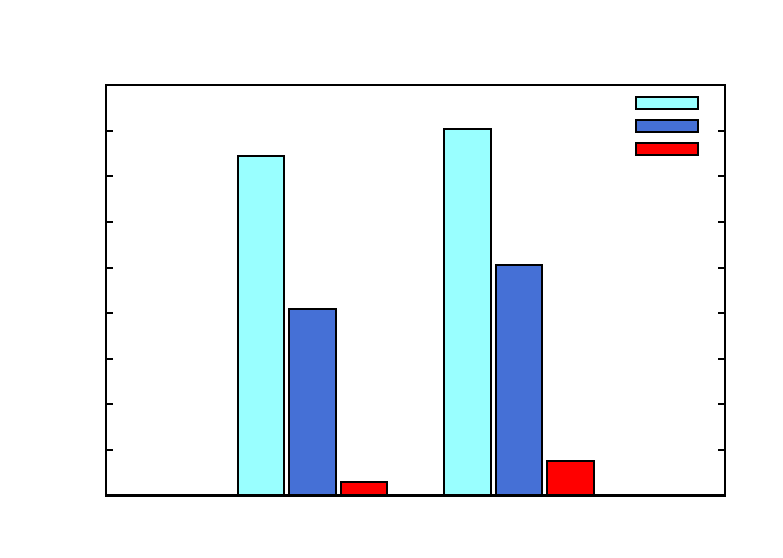
\includegraphics{graph4}}%
    \gplfronttext
  \end{picture}%
\endgroup


% GNUPLOT: LaTeX picture with Postscript
\begingroup
  \makeatletter
  \providecommand\color[2][]{%
    \GenericError{(gnuplot) \space\space\space\@spaces}{%
      Package color not loaded in conjunction with
      terminal option `colourtext'%
    }{See the gnuplot documentation for explanation.%
    }{Either use 'blacktext' in gnuplot or load the package
      color.sty in LaTeX.}%
    \renewcommand\color[2][]{}%
  }%
  \providecommand\includegraphics[2][]{%
    \GenericError{(gnuplot) \space\space\space\@spaces}{%
      Package graphicx or graphics not loaded%
    }{See the gnuplot documentation for explanation.%
    }{The gnuplot epslatex terminal needs graphicx.sty or graphics.sty.}%
    \renewcommand\includegraphics[2][]{}%
  }%
  \providecommand\rotatebox[2]{#2}%
  \@ifundefined{ifGPcolor}{%
    \newif\ifGPcolor
    \GPcolorfalse
  }{}%
  \@ifundefined{ifGPblacktext}{%
    \newif\ifGPblacktext
    \GPblacktexttrue
  }{}%
  % define a \g@addto@macro without @ in the name:
  \let\gplgaddtomacro\g@addto@macro
  % define empty templates for all commands taking text:
  \gdef\gplbacktext{}%
  \gdef\gplfronttext{}%
  \makeatother
  \ifGPblacktext
    % no textcolor at all
    \def\colorrgb#1{}%
    \def\colorgray#1{}%
  \else
    % gray or color?
    \ifGPcolor
      \def\colorrgb#1{\color[rgb]{#1}}%
      \def\colorgray#1{\color[gray]{#1}}%
      \expandafter\def\csname LTw\endcsname{\color{white}}%
      \expandafter\def\csname LTb\endcsname{\color{black}}%
      \expandafter\def\csname LTa\endcsname{\color{black}}%
      \expandafter\def\csname LT0\endcsname{\color[rgb]{1,0,0}}%
      \expandafter\def\csname LT1\endcsname{\color[rgb]{0,1,0}}%
      \expandafter\def\csname LT2\endcsname{\color[rgb]{0,0,1}}%
      \expandafter\def\csname LT3\endcsname{\color[rgb]{1,0,1}}%
      \expandafter\def\csname LT4\endcsname{\color[rgb]{0,1,1}}%
      \expandafter\def\csname LT5\endcsname{\color[rgb]{1,1,0}}%
      \expandafter\def\csname LT6\endcsname{\color[rgb]{0,0,0}}%
      \expandafter\def\csname LT7\endcsname{\color[rgb]{1,0.3,0}}%
      \expandafter\def\csname LT8\endcsname{\color[rgb]{0.5,0.5,0.5}}%
    \else
      % gray
      \def\colorrgb#1{\color{black}}%
      \def\colorgray#1{\color[gray]{#1}}%
      \expandafter\def\csname LTw\endcsname{\color{white}}%
      \expandafter\def\csname LTb\endcsname{\color{black}}%
      \expandafter\def\csname LTa\endcsname{\color{black}}%
      \expandafter\def\csname LT0\endcsname{\color{black}}%
      \expandafter\def\csname LT1\endcsname{\color{black}}%
      \expandafter\def\csname LT2\endcsname{\color{black}}%
      \expandafter\def\csname LT3\endcsname{\color{black}}%
      \expandafter\def\csname LT4\endcsname{\color{black}}%
      \expandafter\def\csname LT5\endcsname{\color{black}}%
      \expandafter\def\csname LT6\endcsname{\color{black}}%
      \expandafter\def\csname LT7\endcsname{\color{black}}%
      \expandafter\def\csname LT8\endcsname{\color{black}}%
    \fi
  \fi
  \setlength{\unitlength}{0.0500bp}%
  \begin{picture}(7200.00,5040.00)%
    \gplgaddtomacro\gplbacktext{%
      \csname LTb\endcsname%
      \put(858,440){\makebox(0,0)[r]{\strut{} 0}}%
      \put(858,1060){\makebox(0,0)[r]{\strut{} 200}}%
      \put(858,1680){\makebox(0,0)[r]{\strut{} 400}}%
      \put(858,2299){\makebox(0,0)[r]{\strut{} 600}}%
      \put(858,2919){\makebox(0,0)[r]{\strut{} 800}}%
      \put(858,3539){\makebox(0,0)[r]{\strut{} 1000}}%
      \put(858,4159){\makebox(0,0)[r]{\strut{} 1200}}%
      \put(2928,220){\makebox(0,0){\strut{}Nodes visited}}%
      \put(4865,220){\makebox(0,0){\strut{}Nodes generated}}%
      \put(3896,4709){\makebox(0,0){\strut{}Results for puzzle 5}}%
    }%
    \gplgaddtomacro\gplfronttext{%
      \csname LTb\endcsname%
      \put(5816,4206){\makebox(0,0)[r]{\strut{}h1}}%
      \csname LTb\endcsname%
      \put(5816,3986){\makebox(0,0)[r]{\strut{}h2}}%
      \csname LTb\endcsname%
      \put(5816,3766){\makebox(0,0)[r]{\strut{}h3}}%
    }%
    \gplbacktext
    \put(0,0){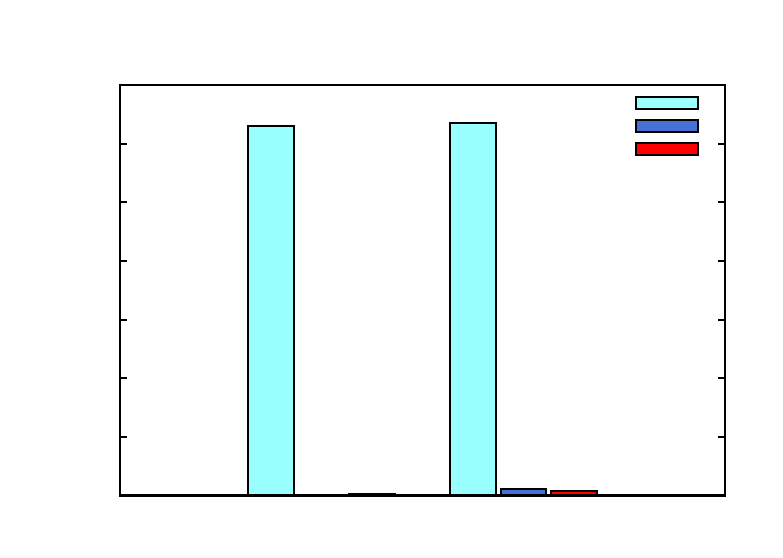
\includegraphics{graph5}}%
    \gplfronttext
  \end{picture}%
\endgroup


\section{Discussions}

The first observation we can make is that the first heuristic generates a huge amount of nodes, more than 1200 for the puzzle 5.
The second heuristic is better, however the number of nodes generated is still huge.
According to our expectations, the third heuristic has the best results.
With this heuristic, the number of nodes generated is only .


For the puzzle 3, we see that the number of nodes generated is less than the number of nodes visited, for all the heuristics.
The explaination is that the initial node is visited, and not expanded.


As a conclusion, this project shows use the importance of the choice of heuristic.
The quality of the heuristic has a huge effect on the performance of the algorithm.


\end{document}
